\documentclass[a4paper,11pt,singlespacing]{article}

\usepackage{setspace}
\usepackage[utf8]{inputenc}
\usepackage[T1]{fontenc}
\usepackage{graphicx}
\usepackage{color}
\usepackage{hyperref}
\usepackage{listings,xcolor}
\usepackage{pdfpages}
\usepackage{float}


\renewcommand{\figurename}{Abbildung}

\graphicspath{ {./images/} }

\title{Hacking von I LOCK IT}
\author{Marius Würstle}
\date{\today}

\begin{document}
	\setlength{\parindent}{0ex}
	\maketitle
	
	\tableofcontents
	\pagebreak
	
	\section{Motivation}
	
	\section{Grundbegriffe}
		CRCInit
		
	
	\section{Problemstellung}
	
	\section{Bluetooth Technologie}
		Bluetooth ist der Industriestandard für die drahtlose Datenübertragung über kurze Distanz. Die Slaves lauschen auf 32 unterschiedlichen Hop-Kanälen, dieser Modus nennt sich Scan-Modus. Der Verbindungsaufbau geht von einem Master Gerät aus und wird mittels einer Inquiry-Nachricht und einer anschließenden Page-Nachricht hergestellt. Falls die Hardware-Adresse(48-Bit lange eindeutige ID) den Geräten bekannt ist wird keine Page Nachricht mehr versendet. In der Page Phase sendet der Master 16 identische Page Nachrichten auf 16 verschiedene Channels. \\
		Bluetooth Low Energy (BLE) wurde für Systeme entwickelt, die auf einem Akku basieren und mit einem möglichst geringen Stromverbrauch funktionieren müssen. Dies wird durch kurze Aktivitätszeiten erreicht, das heißt es wird nur gesendet bzw. gelauscht solange es notwendig ist. Zusätzlich werden die Datenpakete gesammelt und alle zusammen versandt. Darüber hinaus spart die geringe Übertragungsgeschwindigkeit Strom.
		
		\subsection{Advertising}
		BLE nutzt 40 verschieden Channels im Bereich von 2402 MHz bis 2480 MHz. Die einzelnen Channels sind 2 MHz voneinander entfernt, davon werden Channel 37, 38 und 39 nur für das Advertisement verwendet. \\
		Die sogenannten Adveritsements sind die Pakete, die von den Peripherie Geräten ausgesendet werden, um auf sich aufmerksam zu machen. Es gibt noch einige Spezifikationen, der einzelnen Advertisment-Pakete, dies würde allerdings den Rahmen der Arbeit sprengen. Meist sind in diesem Paket der Gerätename, die Service-UUID und die RSSI (RSSI Pegel und Signalstärke). Falls die 31 Bytes an Advertisement-Data des Pakets nicht ausreichen, um alle Informationen zu versenden, kann ein Scan-Request gesendet werden. Welcher logischerweise mit den restlichen Daten in einem Scan-Response beantwortet wird. Allerdings muss das Zentrale System die Anfrage auslösen, um die Daten zu bekommen.
		\begin{figure}[ht]
			\centering
			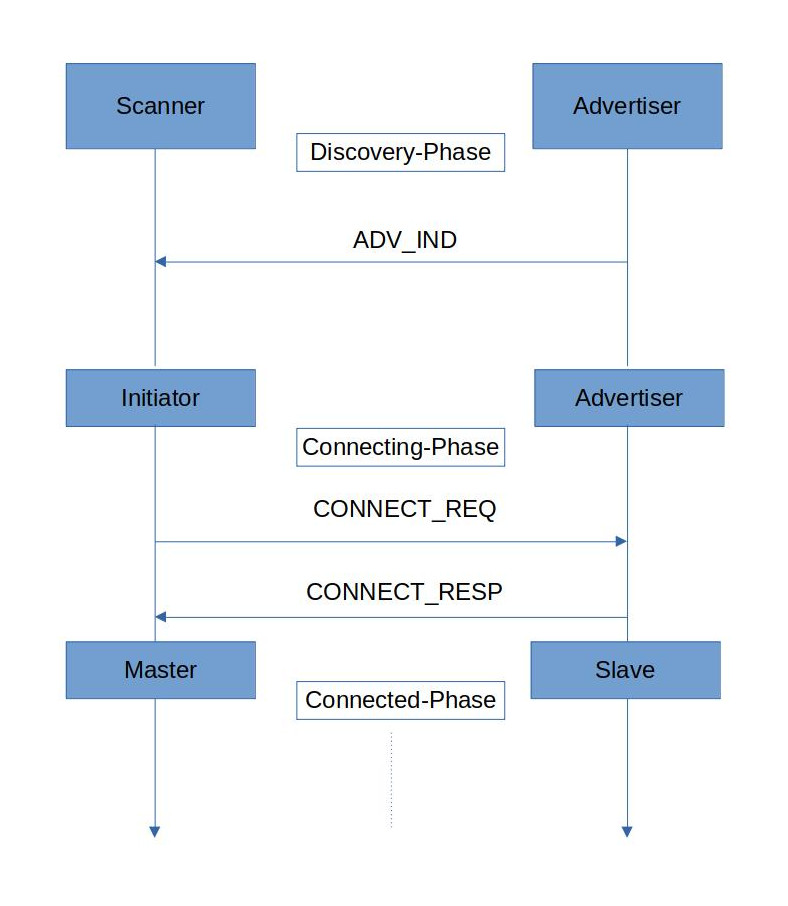
\includegraphics[scale=0.4]{Connection_BLE}
			\caption{Verbindungsaufbau unter BLE}
			\label{connect}
		\end{figure}
		\subsection{Discovery-Phase}
		Die Peripherie Geräte senden ihre Advertisements in dieser Phase auf die 3 oben gennanten Channel mit den auch oben genannten Informationen. Hier könnte auch ein Scan-Request getätigt werden.
		\subsection{Connection-Phase}
		Der Scanner wird jetzt "Initiatior" gennannt und intiert mit einem "CONNECT\_REQ" den Verbindungsaufbau. Dieses Paket beinhaltet die Frequency hopping sequence, Connection Intervall, Slave Latency, Supervision Timeout. Nach dem Versenden oder dem Erhalten dieses Pakets gelten die Systeme als verbunden. \cite{michrochip_dev_connection}
		\subsection{Connected-Phase}
		Nachdem dem Verbindungsaufbau wird der Initiator zum Master und der Advertiser zum Slave und es können Daten ausgetauscht werden. Bei BLE wird dies über den Linked-Layer gemacht, welcher auch verschlüsselt werden kann. Die beiden Geräte tauschen in regelmäßigen Abständen Daten Pakete aus, diese werden "connection events" genannt
		
		\subsection{Security}
		Die Datenpakete können, wie oben schon erwähnt, verschlüsselt werden. Diese Pakete enthalten zusätzlich einen MIC (message Integrity Check), der den Sender authentifiziert. Auch enthält das Paket einen Packet Zähler, um einen replay-Angriff zu verhindern. Verschlüsselt wird mit dem AES-128 Algorithmus und den CCM Modus (Cipher Block Chaining-Message Authentication Code). Eine solche Verbindung kann erst nach dem Aufbau der Connection erstellt werden. Hierfür mussen die geräten sich pairen, wie dies funktioniert gehe ich später ein.
		
		\subsubsection{Pairing}
		Paring wird dann gestartet sobald zwei Geräte miteinander verbunden sind und sie etwas ausführen wollen, dass Security benötigt.\\
		Das Pairning beinhaltet drei wichitige Schritte:
		\begin{itemize}
			\item Authentifizierung von 2 Geräten: \\
			Zu Beginn werden die Input und Output Fähigkeiten der geräte ausgetauscht. Anhand dieser wird ausgewählt wie die Geräte gepaired werden können und welche Art von Keys in der letzten Phase versandt werden.
			\item Erstellen und Austauschen eines Short-Term-Keys(STK): \\
			In diesem Schritt einigen sich die beiden Systeme auf eine Art den STK zu berechnen. Hierbei spielen die I/O Fähigkeiten der Geräte eine große Rolle.
			\item Austauschen eines Long-Term-Keys(LTK): \\
			Zunächst prüft der Intiator, ob das gegenüberliegende Gerät dazu fähig ist sich zu binden. Danach wird der LTK über den durch den STK encrypteten Kanal versendet.
		\end{itemize}
	
	\section{Sicherheitsanalyse}
	
		Herausfinden der encrypt Methode beim Austausch des STK, manche sind nicht MTM sicher?
		
		Untersuchung nach Connection erstellung, ob derk LTK geknackt werden kann?
		
		
	\section{Umsetzung}
		
		Denial of Service Angriff mit BtleJack durch übernahme der Verbindung. (funktioniert schon)
		
	\section{Fazit/Ausblick}
		Nennung der Sicherheitslücken und Ideen wie man diese verhindern kann.
	
	
	
	\bibliography{zitate}
	\bibliographystyle{plain}
	
	
	https://www.rfwireless-world.com/Terminology/BLE-Connection-Establishment-Procedure.html 20 März 2021
	
	https://microchipdeveloper.com/wireless:ble-link-layer-security
	
\end{document}